\documentclass[a4paper,12pt]{beamer}
\usepackage{tabularx}
\usepackage{array}
\usepackage{graphicx}
\usepackage{listings}
\usepackage{hyperref}
\usepackage{color}
\usepackage{tikz}
\usetikzlibrary{arrows.meta, positioning, shapes.geometric,matrix}
\usecolortheme{whale}

\definecolor{lightgray}{gray}{0.95}
\setbeamerfont{section in toc}{size=\small}
\setbeamerfont{subsection in toc}{size=\scriptsize}
\lstset{
    language=SQL,
    showspaces=false, 
    numbers=left,
    numberstyle=\tiny,
    backgroundcolor=\color{lightgray},
    keywordstyle=\color{blue}\bfseries,
    commentstyle=\color{gray},
    stringstyle=\color{orange},
    basicstyle=\ttfamily\scriptsize,
    breaklines=true,
    literate=
        {é}{{\'e}}1
        {è}{{\`e}}1
        {à}{{\`a}}1
        {ù}{{\`u}}1
        {ç}{{\c{c}}}1
        {ô}{{\^o}}1
        {ê}{{\^e}}1,
}

\title{Comment optimiser l'exécution des requêtes SQL sur une base de données?}
\author[Eliott P. \& Antoine BP]{Eliott PAQUET}
\date{2025}
    

% Barre Pied de page
\setbeamertemplate{footline}{
    \begin{beamercolorbox}[wd=\paperwidth,ht=2.5ex,dp=1ex]{author in head/foot}
    \usebeamerfont{author in head/foot}
    \hspace*{2ex}\insertshortauthor\hfill \inserttitle\hfill \insertdate\hfill \insertframenumber/\inserttotalframenumber\hspace*{2ex}
    \end{beamercolorbox}
}

% Barre d'en tête
\setbeamertemplate{headline}{%
    \begin{beamercolorbox}[ht=2.5ex,dp=1.125ex,center]{section in head/foot}
        \insertsection
    \end{beamercolorbox}%
}



\begin{document}
\begin{frame}
    \titlepage\
\end{frame}
\begin{frame}
    \frametitle{Sommaire}
    \tableofcontents[hideallsubsections]
\end{frame}
\AtBeginSection[]{
    \begin{frame}
        \frametitle{Sommaire}
        \tableofcontents[currentsection, hideothersubsections]
    \end{frame}
}


\section{Les bases du traitement des requêtes SQL}
\subsection{Le traitement d'une requête}
\begin{frame}
    \frametitle{Description du traitement d'une requête}
    \begin{figure}[h]
        \centering
        \includegraphics[width=300pt]{ressource/query_map.png}
        \caption{Traitement d'une requête SQL par un SGBD.}
    \end{figure}
\end{frame}
\subsection{l'algèbre relationnelle}
\begin{frame}[fragile]
    \frametitle{Edgar F. Codd (1970)}

    \centering
    Calcul relationnel \(\Longleftrightarrow\) Algèbre relationnelle

    \vspace{0.5cm}

    \begin{minipage}{0.48\textwidth}
        \begin{lstlisting}[language=SQL]
SELECT S.id, S.price
FROM Sales AS S
JOIN Dp ON Dp.id = S.DpId
WHERE Dp.name = 'Morbihan';
            \end{lstlisting}
    \end{minipage}
    \hfill
    \begin{minipage}{0.48\textwidth}
        \centering
        \begin{tikzpicture}[
                scale=0.85,
                transform shape,
                node distance=1cm,
                block/.style={minimum width=1cm, minimum height=1cm, align=center},
                arrow/.style={-Stealth, thick}
            ]

            % Opérateurs
            \node[block] (pi) {$\Pi_{S.id,\,S.price}$};
            \node[block, below=of pi] (sigma) {$\sigma_{Dp.name = \text{'Morbihan'}}$};
            \node[block, below=of sigma] (join) {$\Join_{Dp.id = Sales.DpId}$};

            % Relations
            \node[block, below left=of join] (sales) {$Sales$};
            \node[block, below right=of join] (dp) {$Dp$};

            % Flèches
            \draw[arrow] (sigma) -- (pi);
            \draw[arrow] (join) -- (sigma);
            \draw[arrow] (sales) -- (join);
            \draw[arrow] (dp) -- (join);

        \end{tikzpicture}
    \end{minipage}
\end{frame}

\subsection{La gestion mémoire}
\begin{frame}
    \frametitle{Les bases de données orientées colonnes}
    \begin{figure}[h]
        \centering
        \includegraphics[width=300pt]{ressource/row_vs_column.png}
        \caption{Rendu physique des BDD orientées colonnes et BDD orientées lignes}
    \end{figure}
\end{frame}
\subsection{Notre gestion des tables pendant l'exécution}


\begin{frame}{Notre gestion des tables pendant l'exécution}

    \begin{center}
        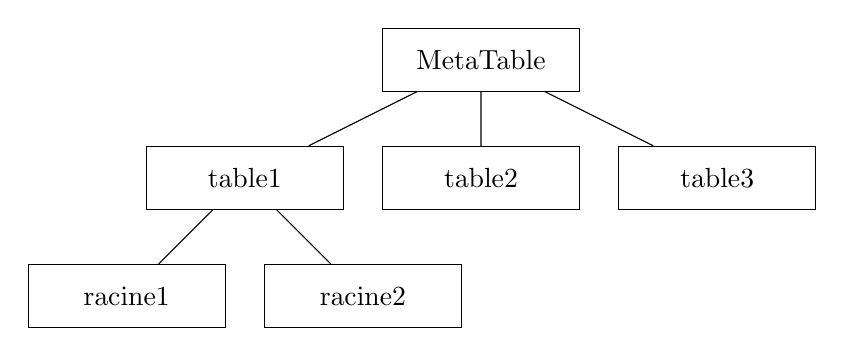
\begin{tikzpicture}[
                level distance=1.5cm,
                sibling distance=3cm,
                every node/.style={draw, rectangle, align=center, minimum width=2.5cm, minimum height=0.8cm}
            ]

            % Racine de l'arbre
            \node {MetaTable}
            % Niveau 1 : les tables
            child { node {table1}
                    % Niveau 2 : racines de table1
                    child { node {racine1} }
                    child { node {racine2} }
                }
            child { node {table2} }
            child { node {table3} };

        \end{tikzpicture}
    \end{center}

    \begin{itemize}
        \item \textbf{Racine}: valeurs chargées.
        \item \textbf{Table}: liste de lignes encore valides.
        \item \textbf{MetaTable}: jointure de plusieurs \textit{Tables}.
        \item \textbf{Particularité}: modifier les lignes d'une \textit{Table} (jointure ou sélection) modifie toutes les \textit{Tables}.
    \end{itemize}

\end{frame}




\section{Les optimisations naïves}
\subsection{La descente des sélections}
\begin{frame}
    \frametitle{La descente des sélections}

    \begin{tikzpicture}[
            scale=0.85,
            transform shape,
            node distance=1cm,
            block/.style={minimum width=1cm, minimum height=1cm, align=center},
            arrow/.style={-Stealth, thick}
        ]

        % Opérateurs
        \node[block] (pi) {$\Pi_{S.id,\,S.price}$};
        \node[block, below=of pi] (sigma) {$\sigma_{Dp.name = \text{'Morbihan'}}$};
        \node[block, below=of sigma] (join) {$\Join_{Dp.id = Sales.DpId}$};

        % Coûts (alignés en face)
        \node[right=1.1cm of pi, anchor=west]    {Coût : $\mathcal{O}(1)$};
        \node[right=1cm of sigma, anchor=west] {Coût : $\mathcal{O}(n)$};
        \node[right=1cm of join, anchor=west]  {Coût : $\mathcal{O}(|\text{Sales}|\times|\text{DP}|)$};

        % Relations
        \node[block, below right=of join] (sales) {$Sales$};
        \node[block, below left=of join] (dp) {$Dp$};

        % Flèches
        \draw[arrow] (sigma) -- (pi);
        \draw[arrow] (join) -- (sigma);
        \draw[arrow] (sales) -- (join);
        \draw[arrow] (dp) -- (join);

    \end{tikzpicture}

\end{frame}


\begin{frame}
    \frametitle{La descente des sélections}

    \begin{tikzpicture}[
            scale=0.85,
            transform shape,
            node distance=1cm,
            block/.style={minimum width=1cm, minimum height=1cm, align=center},
            arrow/.style={-Stealth, thick}
        ]

        % Opérateurs
        \node[block] (pi) {$\Pi_{S.id,\,S.price}$};
        \node[block, below=of pi] (join) {$\Join_{Dp.id = Sales.DpId}$};
        \node[block, below right=of join] (sigma) {$\sigma_{Dp.name = \text{'Morbihan'}}$};

        % Relations
        \node[block, below left=of join] (sales) {$Sales$};
        \node[block, below =of sigma] (dp) {$Dp$};

        % Coûts
        \node[right=1cm of pi, anchor=west]   {Coût : $\mathcal{O}(1)$};
        \node[right=1cm of join, anchor=west] {Coût : $\mathcal{O}(|\text{o(Dp)}|\times|\text{Sales}|)$};
        \node[right=1cm of sigma, anchor=west] {Coût : $\mathcal{O}(|\text{Dp}|)$};

        % Flèches (droites)
        \draw[arrow] (join) -- (pi);
        \draw[arrow] (sigma) -- (join);
        \draw[arrow] (sales) -- (join);
        \draw[arrow] (dp) -- (sigma);

    \end{tikzpicture}

\end{frame}

\begin{frame}
    \begin{figure}[h]
        \centering
        \includegraphics[width=300pt]{ressource/comparaison_0_vs_5.png}

    \end{figure}
\end{frame}

\subsection{Insertion de projections}

\begin{frame}
    \frametitle{Cas problématique}
    \begin{tikzpicture}[
            scale=0.85,
            transform shape,
            node distance=0.9cm and 0.5cm,
            block/.style={minimum width=1.5cm, minimum height=0.5cm, align=center},
            arrow/.style={-Stealth, thick}
        ]

        % Opérateurs en haut
        \node[block] (pi) {$\Pi_{Sales.id, Sales.price}$};

        % Jointures
        \node[block, below=of pi] (join1) {$\Join_{Dp.id = Sales.DpId}$};
        \node[block, below left=of join1] (join2) {$\Join_{Sales.ProductId = Product.id}$};
        \node[block, below right=of join2] (sigma2) {$\sigma_{Product.Price <5}$};
        \node[block, below left=of join2] (sigma) {$\sigma_{Sales.price>100}$};


        % Relations de base
        \node[block, below =of sigma] (sales) {$Sales$};
        \node[block, below =of sigma2] (Product) {$Product$};
        \node[block, below right=of join1] (dp) {$Dp$};

        % Flèches
        \draw[arrow] (join1) -- (pi);
        \draw[arrow] (join2) -- (join1);

        \draw[arrow] (sales) -- (sigma);
        \draw[arrow] (Product) -- (sigma2);
        \draw[arrow] (sigma2) -- (join2);
        \draw[arrow] (sigma) -- (join2);



        \draw[arrow] (dp) -- (join1);

    \end{tikzpicture}
\end{frame}
\begin{frame}
    \frametitle{Insertion utile de la Projection }
    \begin{tikzpicture}[
            scale=0.85,
            transform shape,
            node distance=0.9cm and 0.5cm,
            block/.style={minimum width=1.5cm, minimum height=0.5cm, align=center},
            arrow/.style={-Stealth, thick}
        ]

        % Opérateurs en haut
        \node[block] (pi) {$\Pi_{Sales.id, Sales.price}$};

        % Jointures
        \node[block, below=of pi] (join1) {$\Join_{Dp.id = Sales.DpId}$};
        \node[block,below left=of join1] (pi2) {$\Pi_{Sales.id, Sales.price,Sales.DpId}$};

        \node[block, below =of pi2] (join2) {$\Join_{Sales.ProductId = Product.id}$};
        \node[block, below right=of join2] (sigma2) {$\sigma_{Product.Price <5}$};
        \node[block, below left=of join2] (sigma) {$\sigma_{Sales.price>100}$};


        % Relations de base
        \node[block, below =of sigma] (sales) {$Sales$};
        \node[block, below =of sigma2] (Product) {$Product$};
        \node[block, below right=of join1] (dp) {$Dp$};

        % Flèches
        \draw[arrow] (join1) -- (pi);

        \draw[arrow] (sales) -- (sigma);
        \draw[arrow] (Product) -- (sigma2);
        \draw[arrow] (join2) -- (pi2);
        \draw[arrow] (pi2) -- (join1);

        \draw[arrow] (sigma) -- (join2);
        \draw[arrow] (sigma2) -- (join2);




        \draw[arrow] (dp) -- (join1);

    \end{tikzpicture}
\end{frame}
\begin{frame}
    \begin{figure}[h]
        \centering
        \includegraphics[width=300pt]{ressource/comparaison_0_vs_3.png}
    \end{figure}
\end{frame}
\subsection{Méthodes de jointure}
\begin{frame}
    \frametitle{Les différents types de jointures possibles}
    \begin{itemize}
        \item Produit Cartésien: génère tous les couples possibles et teste la condition de jointure \(\rightarrow O(n^2)\)\\
        \item Jointure Triée: pré-trie les deux tables et lit les deux tables \(\rightarrow o(2n\log(n)+2n)\)
        \item Jointure par dictionnaire: crée un dictionnaire et recherche les correspondances \(\rightarrow O(2n)\)
        \item Leap Frog Trie Join: procédé similaire à la jointure triée mais l'étend à \(k\)-table en simultané\(\rightarrow o(k\times(n\log(n)+n))\).
    \end{itemize}
\end{frame}
\begin{frame}
    \begin{figure}[h]
        \centering
        \includegraphics[width=300pt]{ressource/comparaison_0_vs_4.png}

    \end{figure}
\end{frame}
\section{Optimisation dépendante des données}
\subsection{Optimisation des expression binaire}
\begin{frame}[fragile]
    \frametitle{Analyse des expressions binaires}

    % Query en haut
    \begin{lstlisting}[language=SQL]
Where (Dep.pays = "France" AND Sales.id = 543) OR (Product.Origine = "Chine")
    \end{lstlisting}

    \vspace{0.5cm} % petit espace entre query et arbre

    % Arbre en dessous
    \begin{center}
        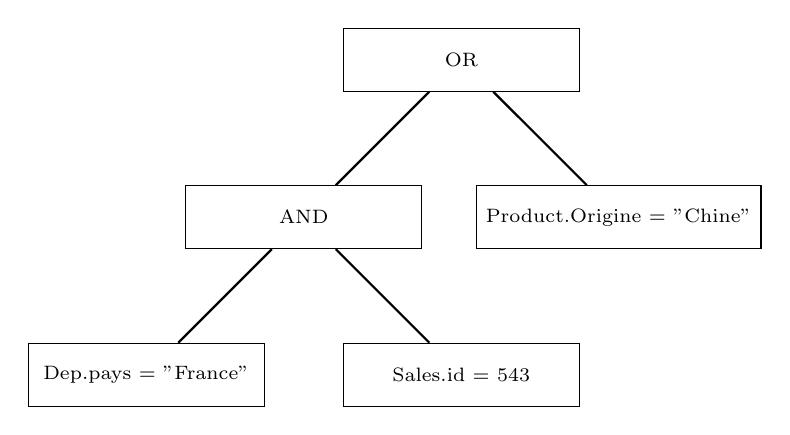
\begin{tikzpicture}[
                scale=1,
                level distance=2cm,
                sibling distance=4cm,
                every node/.style={draw, rectangle, align=center, minimum width=3cm, minimum height=0.8cm, font=\scriptsize},
                arrow/.style={-, thick}]
            % Arbre
            \node (or) {OR}
            child { node (and) {AND}
                    child { node (cond1) {Dep.pays = "France"} }
                    child { node (cond2) {Sales.id = 543} }
                }
            child { node (cond3) {Product.Origine = "Chine"} };

            % Flèches parcours préfixe (parent → enfants)
            \draw[arrow] (or) -- (and);
            \draw[arrow] (and) -- (cond1);
            \draw[arrow] (and) -- (cond2);
            \draw[arrow] (or) -- (cond3);

        \end{tikzpicture}
    \end{center}
\end{frame}

\begin{frame}[fragile]
    \frametitle{Optimisation des expressions binaires}

    % Query en haut
    \begin{lstlisting}[language=SQL]
Where (Dep.pays = "France" AND Sales.id = 543) OR (Product.Origine = "Chine")
    \end{lstlisting}

    \vspace{0.5cm} % petit espace entre query et arbre

    % Arbre en dessous
    \begin{center}
        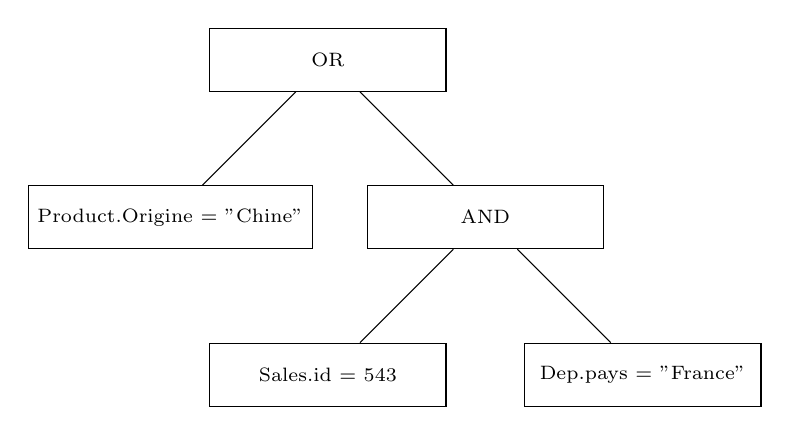
\begin{tikzpicture}[
                scale=1,
                level distance=2cm,
                sibling distance=4cm,
                every node/.style={draw, rectangle, align=center, minimum width=3cm, minimum height=0.8cm, font=\scriptsize},
                arrow/.style={-, thick}]

            % Arbre
            \node (or) {OR}

            child { node (cond3) {Product.Origine = "Chine"} }
            child { node (and) {AND}
                    child { node (cond2) {Sales.id = 543} }
                    child { node (cond1) {Dep.pays = "France"} }
                };

        \end{tikzpicture}
    \end{center}

\end{frame}

\begin{frame}
    \begin{figure}[h]
        \centering
        \includegraphics[width=300pt]{ressource/comparaison_0_vs_2.png}

    \end{figure}
\end{frame}

\subsection{Choix de l'ordre des jointures}
\begin{frame}
    \frametitle{Résultats équivalent mais complexité différente}

    \begin{minipage}{0.48\textwidth}
        \begin{tikzpicture}[
                scale=0.7,
                transform shape,
                node distance=0.6cm and 0cm,
                block/.style={minimum width=0.6cm, minimum height=0.6cm, align=center},
                arrow/.style={-Stealth, thick},
                card/.style={font=\scriptsize, above}
            ]

            % Jointures
            \node[block] (join1) {$\Join_{Dp.id = Sales.DpId}$};
            \node[card] at (join1.north) {$10^2$};

            \node[block, below left=0.8cm and -1cm of join1] (join2)
            {$\Join_{Sales.ProductId = Product.id}$};
            \node[card] at (join2.north) {$10^6$};

            % Relations
            \node[block, below left=0.8cm and -1cm of join2] (sales) {$Sales$};
            \node[card] at (sales.north) {$10^6$};

            \node[block, below right=0.8cm and -1cm of join2] (product) {$Product$};
            \node[card] at (product.north) {$10^4$};

            \node[block, below right=0.8cm and -1cm of join1] (dp) {$Dp$};
            \node[card] at (dp.north) {$1$};

            % Flèches
            \draw[arrow] (join2) -- (join1);
            \draw[arrow] (sales) -- (join2);
            \draw[arrow] (product) -- (join2);
            \draw[arrow] (dp) -- (join1);

        \end{tikzpicture}
    \end{minipage}
    \begin{minipage}{0.48\textwidth}
        \begin{tikzpicture}[
                scale=0.7,
                transform shape,
                node distance=0.6cm and 0cm,
                block/.style={minimum width=0.6cm, minimum height=0.6cm, align=center},
                arrow/.style={-Stealth, thick},
                card/.style={font=\scriptsize, above}
            ]

            % Jointures
            \node[block] (join1) {$\Join_{Sales.ProductId = Product.id}$};
            \node[card] at (join1.north) {$10^2$};

            \node[block, below left=0.8cm and -1cm of join1] (join2)
            {$\Join_{Dp.id = Sales.DpId}$};
            \node[card] at (join2.north) {$10^2$};

            % Relations
            \node[block, below left=0.8cm and -1cm of join2] (sales) {$Sales$};
            \node[card] at (sales.north) {$10^6$};

            \node[block, below right=0.8cm and -1cm of join1] (product) {$Product$};
            \node[card] at (product.north) {$10^4$};

            \node[block, below right=0.8cm and -1cm of join2] (dp) {$Dp$};
            \node[card] at (dp.north) {$1$};

            % Flèches
            \draw[arrow] (join2) -- (join1);
            \draw[arrow] (sales) -- (join2);
            \draw[arrow] (product) -- (join1);
            \draw[arrow] (dp) -- (join2);

        \end{tikzpicture}
    \end{minipage}


    \vspace{1cm}
    \begin{itemize}
        \item \(\Join_{Sales.ProductId = Product.id}\) d'abord → \(10^4\times10^6 + 10^6 \times 1 \) comparaisons
        \item \(\Join_{Dp.id = Sales.DpId}\) d'abord \(\rightarrow\) \(1\times10^6 + 10^2 \times 10^4 \) comparaisons
    \end{itemize}

\end{frame}
\begin{frame}
    \begin{figure}[h]
        \centering
        \includegraphics[width=300pt]{ressource/comparaison_0_vs_1.png}

    \end{figure}
\end{frame}
\subsection{Comment choisir le meilleur plan rapidement?}
\begin{frame}
    \frametitle{Comment choisir le meilleur plan rapidement?}
    \begin{itemize}
        \item Choisir les optimisations avant de lancer la requête
        \item Utiliser l'historique des plans générés
        \item Donner un coût à chaque opération, énumérer tous les plans et prendre celui avec le plus faible coût
    \end{itemize}
\end{frame}

\section{Analyse des résultats}
\subsection{Grand jeux de donnée}
\begin{frame}
    \begin{figure}[h]
        \centering
        \includegraphics[width=300pt]{ressource/toutes_les_courbes.png}
    \end{figure}
\end{frame}
\subsection{Des optimisations impactantes}
\begin{frame}
    \frametitle{Des optimisations impactantes}
    \begin{itemize}
        \item Le choix de la jointure est crucial\\
        \item Il existe un très grand nombre de plan possible et manière de le choisir.
    \end{itemize}
\end{frame}


\subsection{Critique}
\begin{frame}
    \frametitle{Les raisons de la lenteur de notre modèle}
    \begin{itemize}
        \item De nombreuses techniques n'ont pas été traitées, notamment les plus récentes (\(\sim 20\) ans)
        \item Les failles de notre code. \(45\) minutes \(\to\) \(22\) secondes
        \item Les optimisations matérielles. Appel aux fonctions internes au processeur
        \item La compression des données. Exemple: \textit{C-Store} \(4\) manière de compresser les données
        \item La vectorisation et le multi-threading
    \end{itemize}
\end{frame}
\section{Conclusion}
\subsection{Conclusion}
\begin{frame}
    \frametitle{Résumé}
    \begin{itemize}
        \item Les bases des Systèmes de Gestion de Base de Données
        \item Différentes optimisations naïve utilisant l'algèbre relationnelle
        \item Certaines optimisations dépendantes des données que notre SGBD possède
        \item Une analyse des résultats obtenus
    \end{itemize}
\end{frame}
\subsection{Ouverture}
\begin{frame}
    \frametitle{Ouverture}
    \textbf{Les pistes récentes:}
    \begin{itemize}
        \item Analyse des données \(\Rightarrow\) Machine Learning (Génération de plan, Choix de l'ordre des jointures,..)
        \item Une meilleure organisation des données en mémoire (Voire le travail d'Antoine)
        \item Les deux: \href{https://www.normalesup.org/~rouvroy/papers/NTU_25_QHICS.pdf}{\textit{Hypothetical Index Benefit Estimation on Column-oriented Databases using Quantiles} \(2025\)}
        \item Base de donnée sur GPU.SIGMOD de Microsoft

    \end{itemize}

\end{frame}
\subsection{Nos ressources}
\begin{frame}
    \frametitle{Nos ressources}
    \textbf{Nos ressources:}
    \begin{itemize}
        \item \href{https://drive.google.com/file/d/1KNmuRBf8CV-s-zqdkUEP8iyYlPgFiglb/view?usp=drive_link}{\textit{The Design and Implementation of Modern Column-Oriented Database Systems} \(2013\)}
        \item \href{https://web.stanford.edu/class/cs345d-01/rl/cstore.pdf}{\textit{C-Store: A Column-oriented DBMS} \(2005\)}
        \item \href{https://link.springer.com/content/pdf/10.1007/s41019-020-00149-7.pdf}{\textit{A Survey on Advancing the DBMS Query Optimizer: Cardinality Estimation, Cost Model, and Plan Enumeration} \(2021\)}
        \item \href{https://www.microsoft.com/en-us/research/wp-content/uploads/2024/12/Extensible-Query-Optimizers-in-Practice.pdf}{\textit{Extensible Query Optimizers in Practice} \(2024\)}
        \item \href{http://webdam.inria.fr/Alice/}{\textit{Foundation of Databases} \(1995\)}
    \end{itemize}
\end{frame}
\end{document}